\section{Production Deployment: Hardware, Latency, Explainability}
\label{sec:deployment}

Deploying deep learning systems into active high-speed manufacturing environments introduces deterministic physical constraints entirely absent from offline academic research. For capacity planning, a representative cadence of five to thirty components per second implies a nominal latency budget of approximately 30--200\,ms per component. These figures are illustrative engineering assumptions, not measurements from the MVTec evaluation. Each deployment must establish its actual takt time, end-to-end latency budget, and hardware acceptance criteria on the target line.

\subsection{Hardware-Tiered Inference and Cycle-Time Profiling}

The software can select execution settings according to locally available compute resources. The final scientific evaluation establishes detection quality, but it does not constitute a controlled CPU/GPU hardware benchmark.

By standardising on ResNet-18 after Wide-ResNet-50-2 exhausted the development GPU memory during Optuna sweeps, we reduced deployment risk relative to the heavier candidate. Whether feature extraction and nearest-neighbour search meet a plant's throughput target on a fanless Industrial Personal Computer (IPC) remains an acceptance-test question. A retrofit may avoid a dedicated GPU where measured CPU throughput satisfies that line's takt time; otherwise GPU acceleration remains an available deployment option.

Where edge GPU acceleration is present, the same pipeline can use batched execution, subject to target-hardware profiling and end-to-end line validation.

\subsection{Explainable AI (XAI) and Operator Interface Architecture}

An uninterpretable divert signal introduces a severe operational vulnerability: operator override. If line-side quality inspectors cannot discern the physical rationale behind an automated rejection, they routinely dismiss the alert. Over prolonged operations, this breeds chronic skepticism and degrades inspection coverage back to the unreliable manual baseline.

We counteract this vulnerability by providing continuous, pixel-level spatial explainability. Utilising the nearest-neighbour patch distance tensor, our runtime renders a calibrated, colour-coded anomaly heatmap that pinpoints the exact spatial coordinates driving the elevated score. Applying the calibrated decision threshold $\tau$, we derive a binarised defect contour mask, providing the line operator with both an unambiguous anomaly score and an auditable spatial justification. We rescale both outputs to the canonical $256 \times 256$ resolution prior to display, guaranteeing precise geometric alignment with physical part coordinates. Figure~\ref{fig:xai_reconstructions} illustrates representative defect heatmaps and contour overlays.

\begin{figure}[t]
    \centering
    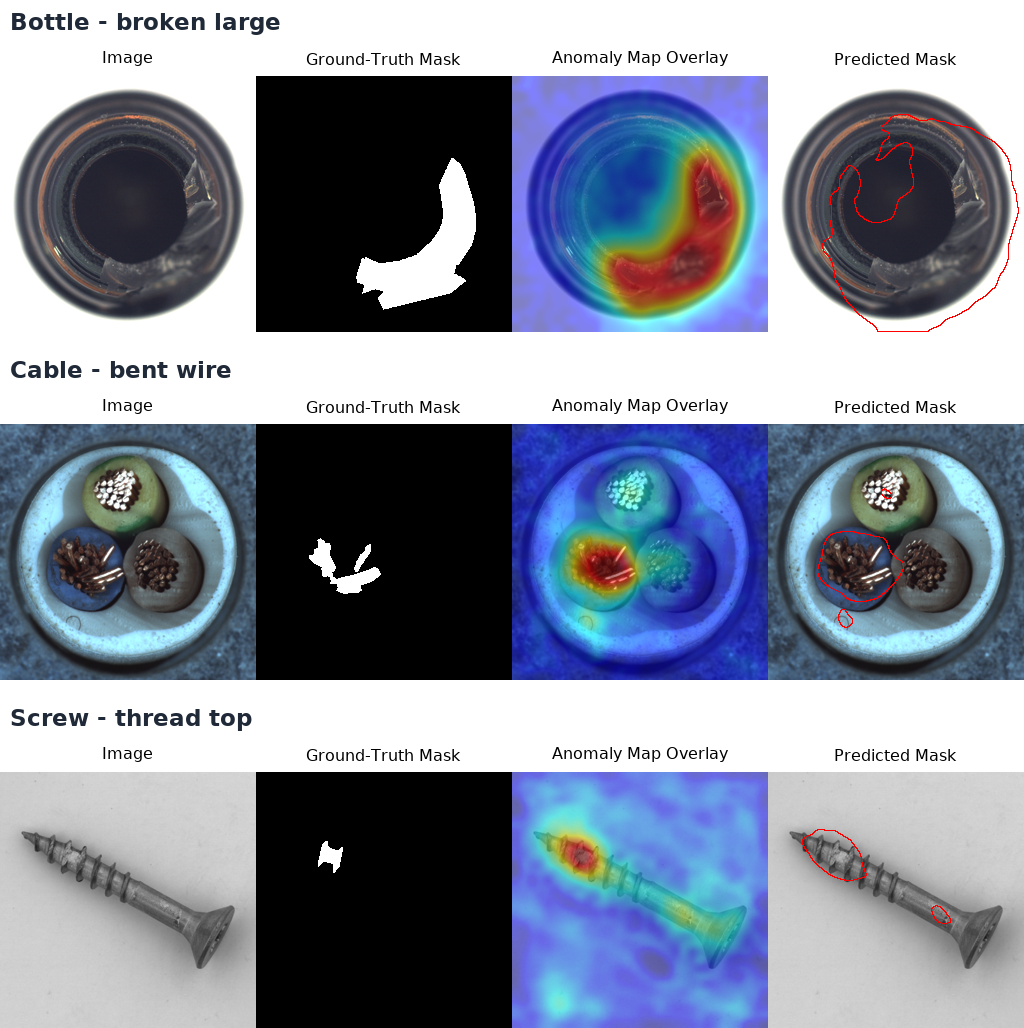
\includegraphics[width=0.88\linewidth]{figures/business_xai_grid.png}
    \caption{Stored PatchCore qualitative outputs for representative Bottle, Cable, and Screw defects. Each row shows the input, ground-truth mask, anomaly-map overlay, and predicted contour mask.}
    \label{fig:xai_reconstructions}
\end{figure}

We deploy the line-side interface as a reactive Streamlit application. Quality engineers can inspect diverted components in real time, examine the spatial heatmap justification, and validate or reclassify the divert. This feedback action appends the verified embeddings to the local memory bank, transforming line operators into active stewards of continuous system refinement whilst requiring zero machine learning background.

\subsection{Enterprise Software Architecture and Intellectual Property Safeguards}

Beyond inference latency, we designed the platform to satisfy rigorous IT governance, reliability, and cybersecurity criteria. We built the platform upon a strictly reproducible software supply chain. We deterministically resolve environment dependencies using \texttt{Pixi}, and orchestrate operational tasks via \texttt{Just}. This guarantees that software installations execute deterministically across distributed edge nodes without library collisions.

Furthermore, we adhere to strict corporate IP and legal compliance standards. We constructed the core runtime exclusively upon permissively licensed, enterprise-compliant open-source frameworks (notably PyTorch and Anomalib \cite{anomalib} under Apache 2.0 and MIT licences). We strictly exclude viral copyleft licences (such as GPL/AGPL) that could legally threaten client intellectual property. This guarantees legal security for corporate procurement and ensures that manufacturing designs remain strictly confidential.
